 \documentclass[11pt]{article}

\usepackage{latexsym}
\usepackage{amssymb}
\usepackage{amsthm}
\usepackage{amscd}
\usepackage{amsmath}
\usepackage{tikz}
\usepackage{graphicx}
\usepackage[final]{pdfpages}
\usepackage{enumerate}

\newcommand{\ZZ}{\mathbb{Z}}

\setlength{\evensidemargin}{1in}
\addtolength{\evensidemargin}{-1in}
\setlength{\oddsidemargin}{1.5in}
\addtolength{\oddsidemargin}{-1.5in}
\setlength{\topmargin}{1in}
\addtolength{\topmargin}{-1.5in}

\setlength{\textwidth}{16cm}
\setlength{\textheight}{23cm}

\newcommand{\rook}{\hspace{-.1cm}\amalg\hspace{-.15cm}\bar{}}
\newcommand{\Stab}{\mathrm{Stab}}
\newcommand{\FF}{\mathbb{F}}


\begin{document}
\begin{center}
\section*{William Daniels}
\section*{CSCI 4202}
\subsection*{Artificial Intelligence}
\subsection*{Homework \#7 03/16/15}
\end{center}

\vspace{.25cm}

The first problem uses the regular (non-stack) STRIPS Approach. Below you'll find a pdf insert of the solution (created this way for easier viewing, starts on the next page):

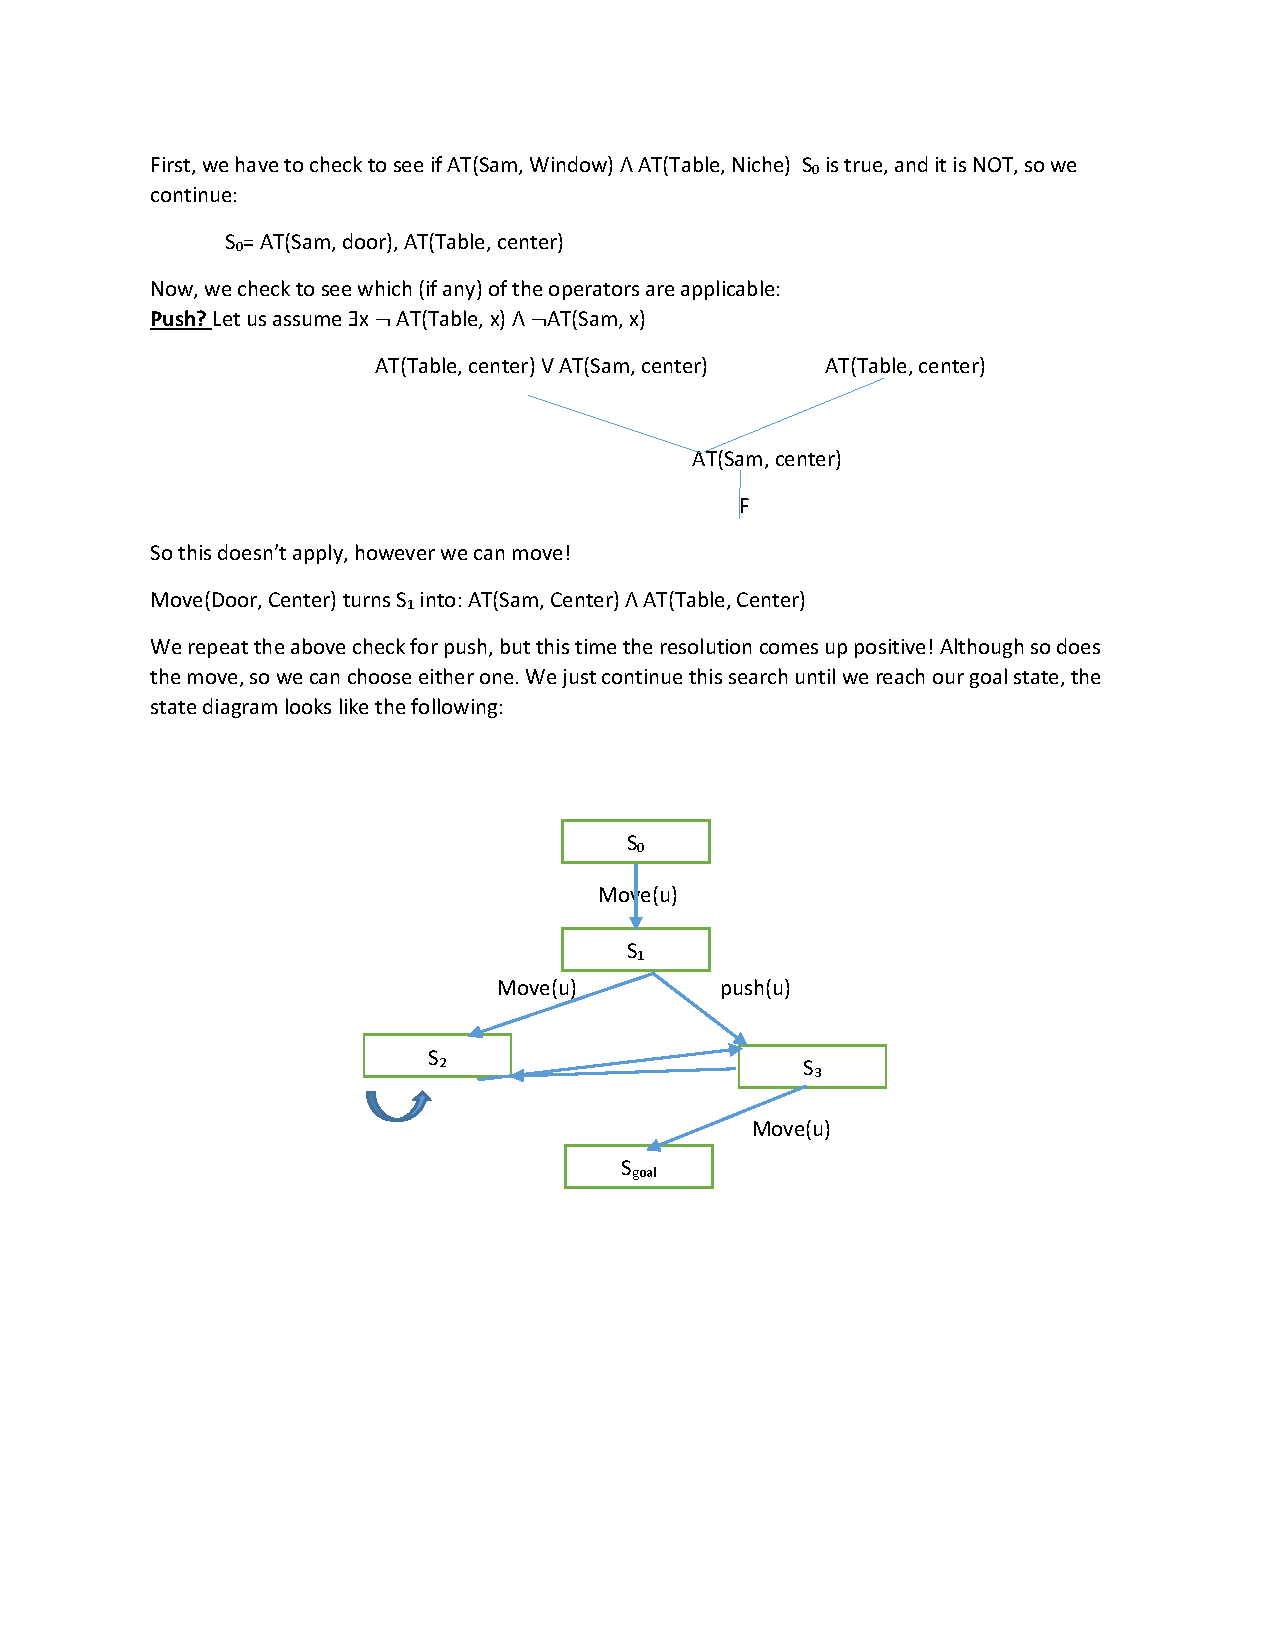
\includepdf[pages=1]{StripsRegular.pdf}



\end{document}

